\begin{frame}{Reading Model}

\centering
\usetikzlibrary{shapes.misc}

\begin{adjustbox}{max width=\linewidth, max height=\textheight, keepaspectratio}
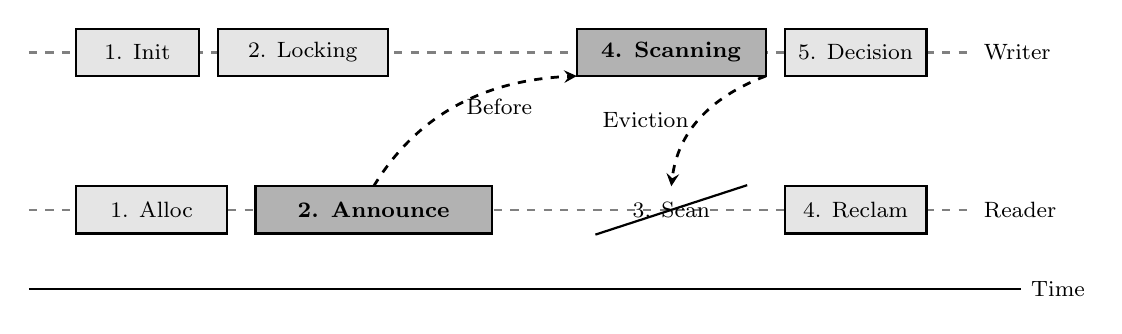
\begin{tikzpicture}[
    xscale=1.2, yscale=1.0, every node/.style={font=\footnotesize},
    cNode/.style={circle, draw, minimum size=15mm, fill=black!10, thick, font=\small},
    sNode/.style={rectangle, draw, minimum width=15mm, minimum height=2mm, fill=black!30, thick},
    edge/.style={draw, thick},
    fStyle/.style={draw=black, ultra thick, dashed, fill=blue!5, fill opacity=0.1, rounded corners=3mm, inner sep=3mm},
    phaseNorm/.style={rectangle, draw, thick, fill=black!10, minimum height=6mm},
    phaseBold/.style={rectangle, draw, thick, fill=black!30, minimum height=6mm}
]
    \draw[gray, dashed, thick] (0,1.5) -- (10.0,1.5) node[right, black] {Writer};
    \draw[phaseNorm] (0.5,1.2) rectangle (1.8,1.8) node[pos=.5] {1. Init};
    \draw[phaseNorm] (2.0,1.2) rectangle (3.8,1.8) node[pos=.5] {2. Locking};
    \draw[phaseBold] (5.8,1.2) rectangle (7.8,1.8) node[pos=.5] {\textbf{4. Scanning}};
    \draw[phaseNorm] (8.0,1.2) rectangle (9.5,1.8) node[pos=.5] {5. Decision};

    \draw[gray, dashed, thick] (0,-0.5) -- (10.0,-0.5) node[right, black] {Reader};
    \draw[phaseNorm] (0.5,-0.8) rectangle (2.1,-0.2) node[pos=.5] {1. Alloc};
    \draw[phaseBold] (2.4,-0.8) rectangle (4.9,-0.2) node[pos=.5] {\textbf{2. Announce}};

    \node[draw, thick, fill=black!10, cross out, strike out, minimum width=1.9cm, minimum height=0.6cm] at (6.8,-0.5) {};
    \node at (6.8,-0.5) {3. Scan};

    \draw[phaseNorm] (8.0,-0.8) rectangle (9.5,-0.2) node[pos=.5] {4. Reclam};

    \draw[edge] (0,-1.5) -- (10.5,-1.5) node[right] {Time};

    \draw[->, >=stealth, line width=1pt, dashed, black] (3.65,-0.2) to [bend left=30] node[right, midway] {Before} (5.8,1.2);

    \draw[->, >=stealth, line width=1pt, dashed, black] (7.8,1.2) to [bend right=30] node[left, midway, align=right] {Eviction} (6.8,-0.2);
\end{tikzpicture}
\end{adjustbox}

\vspace{1.0cm}

\begin{adjustbox}{max width=\linewidth, max height=\textheight, keepaspectratio}
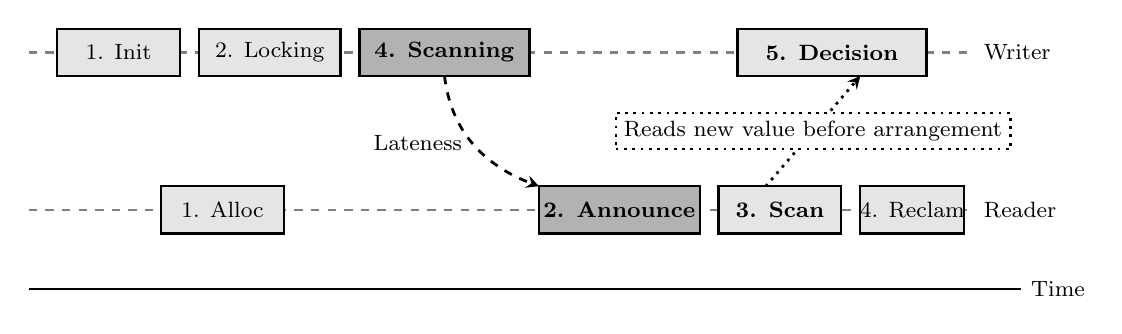
\begin{tikzpicture}[
    xscale=1.2, yscale=1.0, every node/.style={font=\footnotesize},
    cNode/.style={circle, draw, minimum size=15mm, fill=black!10, thick, font=\small},
    sNode/.style={rectangle, draw, minimum width=15mm, minimum height=2mm, fill=black!30, thick},
    edge/.style={draw, thick},
    fStyle/.style={draw=black, ultra thick, dashed, fill=blue!5, fill opacity=0.1, rounded corners=3mm, inner sep=3mm},
    phaseNorm/.style={rectangle, draw, thick, fill=black!10, minimum height=6mm},
    phaseBold/.style={rectangle, draw, thick, fill=black!30, minimum height=6mm}
]
    \draw[gray, dashed, thick] (0,1.5) -- (10.0,1.5) node[right, black] {Writer};
    \draw[phaseNorm] (0.3,1.2) rectangle (1.6,1.8) node[pos=.5] {1. Init};
    \draw[phaseNorm] (1.8,1.2) rectangle (3.3,1.8) node[pos=.5] {2. Locking};
    \draw[phaseBold] (3.5,1.2) rectangle (5.3,1.8) node[pos=.5] {\textbf{4. Scanning}};
    \draw[phaseNorm] (7.5,1.2) rectangle (9.5,1.8) node[pos=.5] {\textbf{5. Decision}};

    \draw[gray, dashed, thick] (0,-0.5) -- (10.0,-0.5) node[right, black] {Reader};
    \draw[phaseNorm] (1.4,-0.8) rectangle (2.7,-0.2) node[pos=.5] {1. Alloc};
    \draw[phaseBold] (5.4,-0.8) rectangle (7.1,-0.2) node[pos=.5] {\textbf{2. Announce}};
    \draw[phaseNorm] (7.3,-0.8) rectangle (8.6,-0.2) node[pos=.5] {\textbf{3. Scan}};
    \draw[phaseNorm] (8.8,-0.8) rectangle (9.9,-0.2) node[pos=.5] {4. Reclam};

    \draw[edge] (0,-1.5) -- (10.5,-1.5) node[right] {Time};

    \draw[->, >=stealth, line width=1pt, dashed, black] (4.4,1.2) to [bend right=30] node[left, midway, align=right] {Lateness} (5.4,-0.2);

    \draw[->, >=stealth, line width=1pt, black, dotted] (7.8,-0.2) -- (8.8,1.2)
        node[midway, fill=white, draw=black, thick, inner sep=3pt, align=center] {Reads new value before arrangement};
\end{tikzpicture}
\end{adjustbox}


\textit{Strategy for linearization point}

\note{Here we see two main behaviors of this system. In the first case, the writing thread aborts the read operation since it changed the state. We don't care about the specific implementation; what matters is that it can be done efficiently using CAS}

\note{In the second scenario, the writer is late, shifting linearizability careness to the reader. Thus, reading before the \texttt{Decision} phase yields the old value; otherwise, it returns the new one, as if already updated in memory}

\end{frame}
